\documentclass{article}
\usepackage[utf8]{inputenc}           % Use uft8 enconding to have a wide
                                      % number of symbols available
\usepackage[spanish]{babel}           % Configure the text language
                                      % to know where to put the hyphen in a 
                                      % line break
\usepackage{graphicx}                 % To include images
\usepackage{anysize}                  % Allows marginsize command
\usepackage{fancyhdr}                 % Configure the header and footer  
\usepackage{titlesec}                 % Changes the section titles properties
\usepackage{amsmath}                  % Active wide number of math symbols
\usepackage{amssymb}                  % Math symbols such as semijoin
\usepackage{longtable}                % Multiple-page table
\usepackage[export]{adjustbox}        % Allows to resize tables
\usepackage{enumitem}                 % Controls the item position 
\usepackage{listings}                 % Package for code fences
%\usepackage{xcolor}                   % Create colors
\usepackage[
  table,
  svgnames,
  dvipsnames
]{xcolor}                             % Colors for code fences and 
                                      %table (rowcolor)
\usepackage{textcomp}                 % Helps to display quotes symbols properly
\usepackage{array}                    % Align fix size columns in tables

\decimalpoint%                        % Use dot instead of comma to write 
                                      % decimal numbers
\setlength{\parindent}{0in}           % No indentation at first paragraph

\renewcommand{\familydefault}{\sfdefault} % Changing font
\titleformat*{\section}{\large\bfseries}  % Change section size
\marginsize{1.5cm}{2cm}{1.2cm}{1cm}       % {left}{right}{above}{below}
\setlength{\headsep}{0.3in}               % Changing headsep length
                                          % headsep is the vertical length 
                                          % between header an text area
\lstset{upquote=true}                     % For display quotes and double 
                                          % quoutes in a better style

% Defining column content alignment for fix size columns
\newcolumntype{L}[1]{>{\raggedright\let\newline\\\arraybackslash\hspace{0pt}}m{#1}}
\newcolumntype{C}[1]{>{\centering\let\newline\\\arraybackslash\hspace{0pt}}m{#1}}
\newcolumntype{R}[1]{>{\raggedleft\let\newline\\\arraybackslash\hspace{0pt}}m{#1}}  

%%%%%%%%%%%%%%%%%%%%%%%%%%%%%%%%%%%%%%%%%%%%%%%%%%%%%%%%%%%%%%%%%%%%%%%%%%%%%%%
%%%%%%%%%%                        Code style                         %%%%%%%%%%
%%%%%%%%%%%%%%%%%%%%%%%%%%%%%%%%%%%%%%%%%%%%%%%%%%%%%%%%%%%%%%%%%%%%%%%%%%%%%%%

\definecolor{codegreen}{rgb}{0,0.6,0}
\definecolor{codegray}{rgb}{0.5,0.5,0.5}
\definecolor{codepurple}{rgb}{0.58,0,0.82}
\definecolor{backcolour}{rgb}{1,1,1}

\lstdefinestyle{mystyle}{
  backgroundcolor=\color{backcolour},   
  commentstyle=\color{codegreen},
  keywordstyle=\color{magenta},
  numberstyle=\tiny\color{codegray},
  stringstyle=\color{codepurple},
  %
  basicstyle=\ttfamily\footnotesize,
  captionpos=b,                    
  breakatwhitespace=false,         
  breaklines=true,                 
  keepspaces=true,                 
  showspaces=false,                
  showstringspaces=false,
  showtabs=false,                  
  %
  tabsize=2
  % Diplay number to the left
  % numbers=left,                    
  % numbersep=5pt,                  
}

\lstset{style=mystyle}


%%%%%%%%%%%%%%%%%%%%%%%%%%%%%%%%%%%%%%%%%%%%%%%%%%%%%%%%%%%%%%%%%%%%%%%%%%%%%%%
%%%%%%%%%%                        Header Style                       %%%%%%%%%%
%%%%%%%%%%%%%%%%%%%%%%%%%%%%%%%%%%%%%%%%%%%%%%%%%%%%%%%%%%%%%%%%%%%%%%%%%%%%%%%

\pagestyle{fancy}
\fancyhf{}
\renewcommand{\headrulewidth}{0pt}

% Right header
% The right header has 
%   the subject title,
%   subtitle and 
%   the university logo
\fancyhead[R]{
    \begin{tabular}{l}
        \materia \\ 
        \actividad%
    \end{tabular}
    \,% Adding space between titles and logo    
    \rule[-1.75\baselineskip]{0pt}{0pt}
    % Strut to ensure a 1/4 \baselineskip between image and header rule
    
\includegraphics[height=3\baselineskip,valign=c]{unam}
}

%%%%%%%%%%%%%%%%%%%%%%%%%%%%%%%%%%%%%%%%%%%%%%%%%%%%%%%%%%%%%%%%%%%%%%%%%%%%%%%
%%%%%%%%%%              Cover page generator command                 %%%%%%%%%%
%%%%%%%%%%%%%%%%%%%%%%%%%%%%%%%%%%%%%%%%%%%%%%%%%%%%%%%%%%%%%%%%%%%%%%%%%%%%%%%

\newcommand{\coverPage}{
\thispagestyle{empty}
  \begin{minipage}[t][5cm][t]{0.2\linewidth}
    
\includegraphics[width=2.5cm]{unam.jpg}

    \vspace{10cm}
    % The following space is mandatory to display correct layout

    
\includegraphics[width=2.5cm]{fiblack}
  \end{minipage}
  %
  \begin{minipage}[t]{0.7\linewidth}
    \vspace{-2.5cm}
    \LARGE{\textbf{\university}}\\
    \Large{\textbf{\faculty}} \\
  
    \large{\semestre}\\[2cm]
  
    \large{\textbf{\materia (\clave)}}\\
    \large{\textbf{Gpo: \grupo}}\\[5mm]
    \large{\textbf{Profesor:} \profesor}\\ [1.5cm]
    \begin{center}
        \LARGE{\textbf{\actividad}}\\
        \LARGE{\textbf{\titulo}}\\
    \end{center}
  
    \vspace{3.3cm}
  
    %\large{\textbf{Alumno:} \alumno} \\[1.5cm]
    \large{
      \begin{itemize}[ noitemsep, align=left ]
        \item [\textbf{Alumno(s):}] 
          \begin{flushright}
            \alumno
          \end{flushright}
      \end{itemize}
    } \vspace{1.5cm}
  
    \begin{flushright}
        \fechaEntrega%
    \end{flushright}
  \end{minipage}

\newpage
}

\begin{document}

%%%%%%%%%%%%%%%%%%%%%%%%%%%%%%%%%%%%%%%%%%%%%%%%%%%%%%%%%%%%%%%%%%%%%%%%%%%%%%%
%%%%%%%%%%                Variables definition                       %%%%%%%%%%
%%%%%%%%%%%%%%%%%%%%%%%%%%%%%%%%%%%%%%%%%%%%%%%%%%%%%%%%%%%%%%%%%%%%%%%%%%%%%%%

\newcommand{\university}{Universidad Nacional Autónoma de México}
\newcommand{\faculty}{Facultad de Ingeniería}
\newcommand{\semestre}{2021-1}
\newcommand{\materia}{BDD}
\newcommand{\clave}{294}
\newcommand{\grupo}{1}
\newcommand{\profesor}{Ing. Rodriguez Campos \textsc{Jorge Alberto}}

%\newcommand{\alumno}{Francisco Pablo \textsc{Rodrigo}}
\newcommand{\alumno}{
  Francisco Pablo \textsc{Rodrigo} \\ 
  Flores Martinez \textsc{Emanuel}   
}
\newcommand{\actividad}{Práctica Final}
\newcommand{\titulo}{BDD empleada para administrar ventas de autos}

\newcommand{\fechaEntrega}{}

\newcommand{\codedir}{codigo}
\graphicspath{{assets/}{bdd_proyecto.assets/}{modelo}}

\coverPage%


%%%%%%%%%%%%%%%%%%%%%%%%%%%%%%%%%%%%%%%%%%%%%%%%%%%%%%%%%%%%%%%%%%%%%%%%%%%%%%%
%%%%%%%%%%                        Contents                           %%%%%%%%%%
%%%%%%%%%%%%%%%%%%%%%%%%%%%%%%%%%%%%%%%%%%%%%%%%%%%%%%%%%%%%%%%%%%%%%%%%%%%%%%%

\section*{Modelo relacional global}

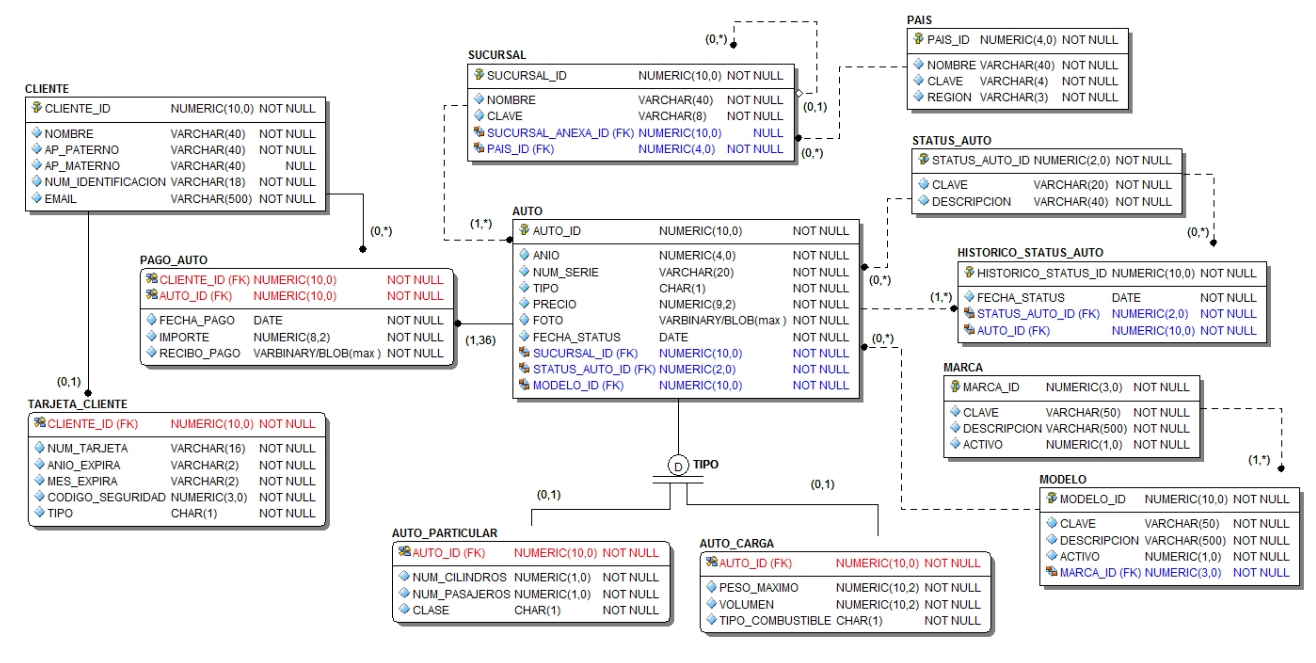
\includegraphics[width=\linewidth]{modelo}\\

\section*{Modelo relacional local de cada sitio}

\subsection*{Sitio 1}
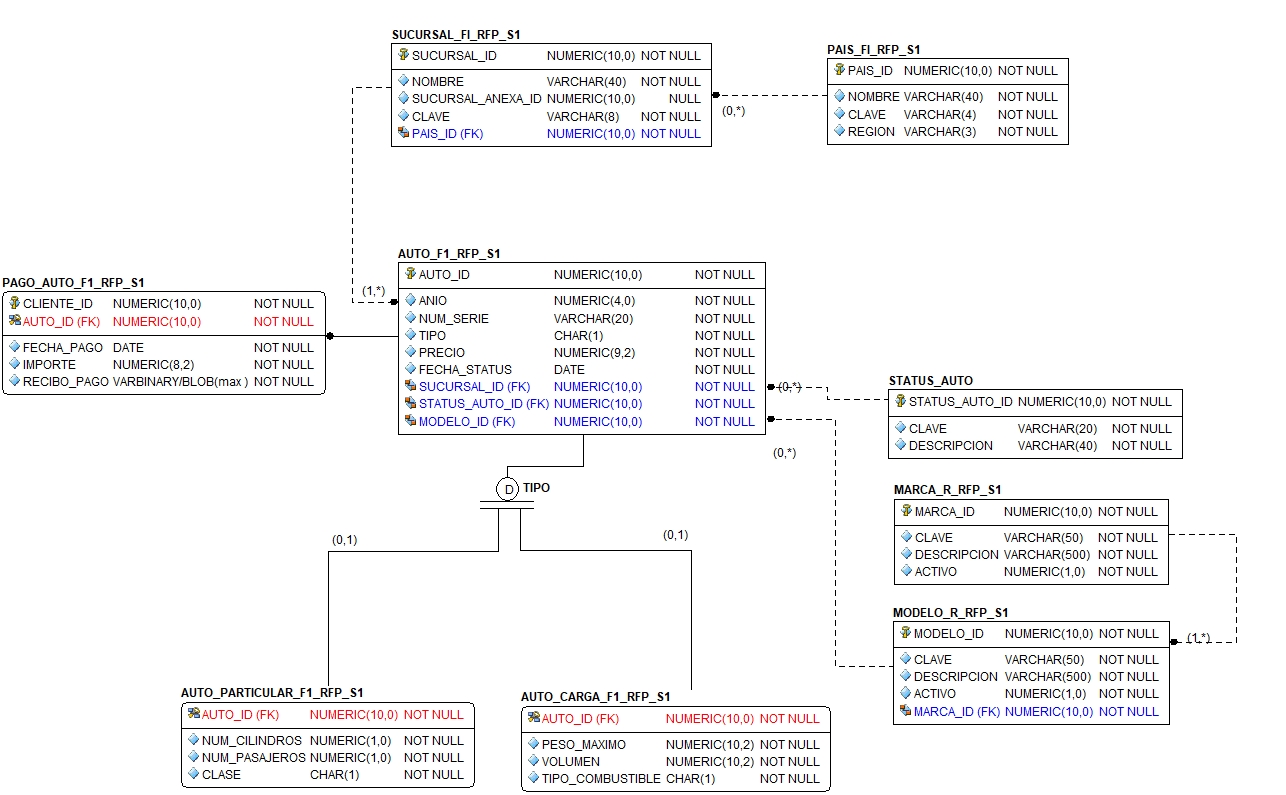
\includegraphics[width=\linewidth]{modelo-n1}\\
\subsection*{Sitio 2}
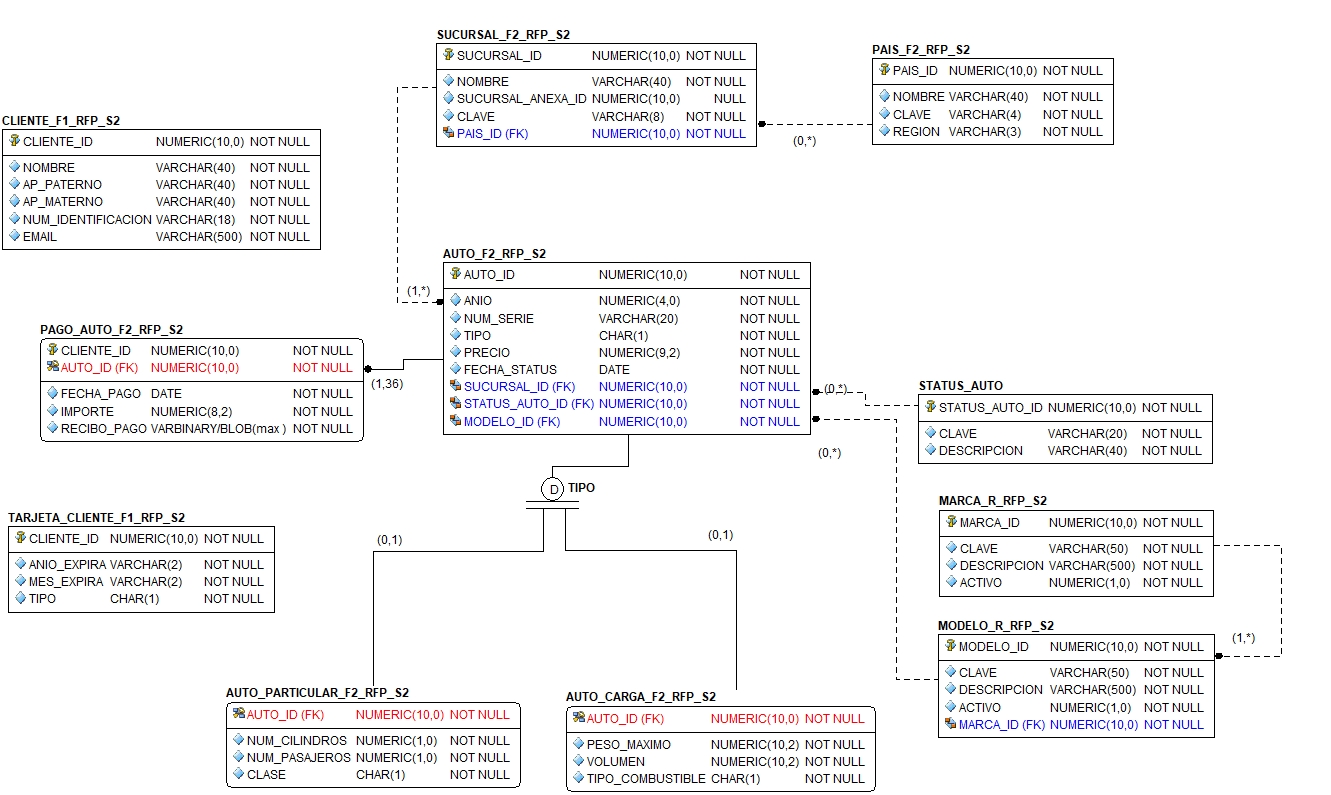
\includegraphics[width=\linewidth]{modelo-n2}\\
\subsection*{Sitio 3}
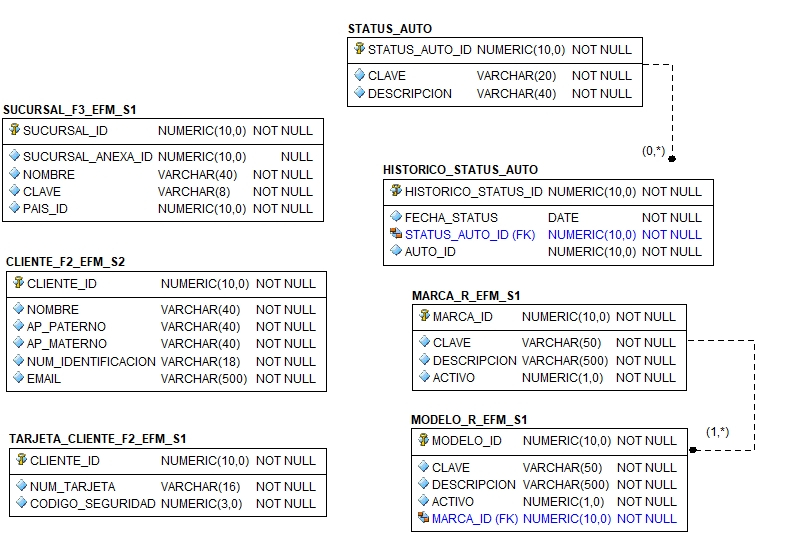
\includegraphics[width=0.8\linewidth]{modelo-n3}\\
\subsection*{Sitio 4}
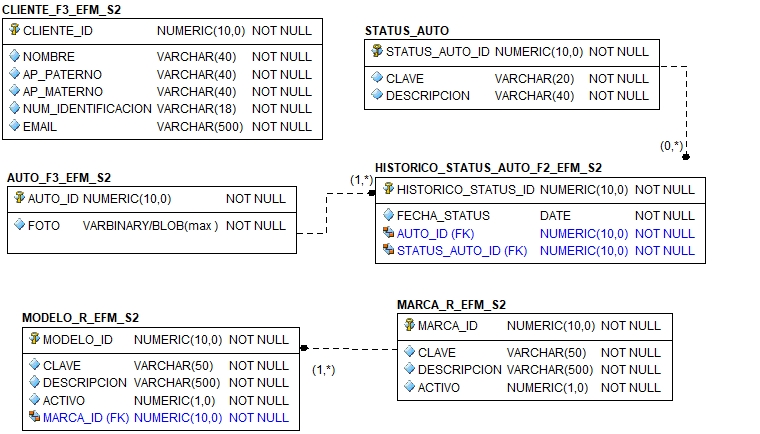
\includegraphics[width=0.8\linewidth]{modelo-n4}

\section*{Tabla de asignación de sitios}

\newcounter{nodeCounter}
\newcommand{\nameTabBuilder}[1]{F\_RFP\_#1}
\newcommand{\snI}{RFP\_S1}
\newcommand{\snII}{RFP\_S2}
\newcommand{\snIII}{EFM\_S1}
\newcommand{\snIV}{EFM\_S2}
\newcommand{\pdbI}{rfpbd\_s1.fi.unam}
\newcommand{\pdbII}{rfpbd\_s2.fi.unam}
\newcommand{\pdbIII}{efmbd\_s1.fi.unam}
\newcommand{\pdbIV}{efmbd\_s2.fi.unam}

{
  \setlength\tabcolsep{3.5mm}
  \def\arraystretch{2}          % Do not define globally (for that reason we
                                % enclose table inside brackets)
  \begin{longtable}{
    |C{0.05\linewidth}
    |p{0.5\linewidth}
    |C{0.2\linewidth}
    |p{0.1\linewidth}|}
  \hline
  %%%%% Start: Table header 
  \textbf{Núm. nodo} &
  \textbf{Características} & 
  \textbf{Nombre global del PDB} & 
  \parbox[t]{2cm}{\centering \textbf{Sufijo para fragmentos}} 
  \\ \hline
  %%%%% End: Table header 
  %
  % row 1
  \stepcounter{nodeCounter} \arabic{nodeCounter} &
  Se encuentra en la región AME y es el servidor con la mayor capacidad 
  de procesamiento & 
 \pdbI & 
  \snI 
  \\ \hline
  %
  % row 2
  \stepcounter{nodeCounter} \arabic{nodeCounter} &
  Se encuentra en la región EUR & 
  \pdbII & 
  \snII
  \\ \hline
  %
  % row 3
  \stepcounter{nodeCounter} \arabic{nodeCounter} &
  Cuenta con una VPN que conecta al servidor con las oficinas de los dueños de 
  la empresa, así como herramientas para cifrado de datos. Se encuentra en las 
  oficinas centrales de la empresa en USA. & 
  \pdbIII & 
  \snIII
  \\ \hline
  %
  % row 4
  \stepcounter{nodeCounter} \arabic{nodeCounter} &
  Cuenta con herramientas para realizar procesamiento de contenido multimedia. 
  Así como una gran capacidad de almacenamiento. Se encuentra en las oficinas 
  centrales de la empresa en USA. & 
  \pdbIV & 
  \snIV
  \\ \hline
  \end{longtable}
}

\section*{Tabla de fragmentación}

\newcounter{fragmentCounter}
\newcommand{\tx}[1]{\text{#1}}   

% Declaring table name variable to reuse them
\newcommand{\cpm}{COPIA MANUAL}
\newcommand{\tbr}{TABLA REPLICADA}
\newcommand{\pais}{PAIS}
\newcommand{\sucursal}{SUCURSAL}
\newcommand{\auto}{AUTO}
\newcommand{\sauto}{STATUS\_AUTO}
\newcommand{\cliente}{CLIENTE}
\newcommand{\autop}{AUTO\_PARTICULAR}
\newcommand{\autoc}{AUTO\_CARGA}
\newcommand{\pagoa}{PAGO\_AUTO}
\newcommand{\tarjeta}{TARJETA\_CLIENTE}
\newcommand{\historico}{HISTORICO\_STATUS\_AUTO}
\newcommand{\fragNameBuilder}[3]{#1\_#2\_#3}      % Params:
                                                  % #1: table name
                                                  % #2: pdb
                                                  % #3: node

{
  \setlength\tabcolsep{1mm}
  \def\arraystretch{2}          % Do not define globally (for that reason we
                                % enclose table inside brackets)
  \begin{longtable}{
    |C{0.075\linewidth}
    |C{0.3\linewidth}
    |C{0.6\linewidth}|}
  \hline
  %%%%% Start: Table header 
  \textbf{Núm frag.} &
  \textbf{Nombre del fragmento} &
  \textbf{Expresión algebraica} 
  \\ \hline
  %%%%% End: Table header 
  %
  % row 1
  \stepcounter{fragmentCounter} \arabic{fragmentCounter} &
  \sauto & 
  \cpm 
  \\ \hline
  %
  % row 2
  \stepcounter{fragmentCounter} \arabic{fragmentCounter} &
  MARCA\_R\_\snI & 
  \tbr 
  \\ \hline
  %
  % row 3
  \stepcounter{fragmentCounter} \arabic{fragmentCounter} &
  MARCA\_R\_\snII & 
  \tbr 
  \\ \hline
  %
  % row 4
  \stepcounter{fragmentCounter} \arabic{fragmentCounter} &
  MARCA\_R\_\snI & 
  \tbr 
  \\ \hline
  %
  % row 5
  \stepcounter{fragmentCounter} \arabic{fragmentCounter} &
  MARCA\_R\_\snII & 
  \tbr 
  \\ \hline
  %
  % row 6
  \stepcounter{fragmentCounter} \arabic{fragmentCounter} &
  MODELO\_R\_\snI & 
  \tbr 
  \\ \hline
  %
  % row 7
  \stepcounter{fragmentCounter} \arabic{fragmentCounter} &
  MODELO\_R\_\snII & 
  \tbr 
  \\ \hline
  %
  % row 8
  \stepcounter{fragmentCounter} \arabic{fragmentCounter} &
  MODELO\_R\_\snI & 
  \tbr 
  \\ \hline
  %
  % row 9
  \stepcounter{fragmentCounter} \arabic{fragmentCounter} &
  MODELO\_R\_\snII & 
  \tbr 
  \\ \hline  
  %
  % row 10
  \stepcounter{fragmentCounter} \arabic{fragmentCounter} &
  \fragNameBuilder{\pais}{F1}{\snI} &
  \begin{minipage}[b]{\linewidth}
    \begin{equation*}
      \sigma_{\tx{clave $=$ `AME'}}(\tx{\pais})  
    \end{equation*} 
  \end{minipage} 
  \\ \hline  
  %
  % row 11
  \stepcounter{fragmentCounter} \arabic{fragmentCounter} &
  \fragNameBuilder{\pais}{F2}{\snII} &
  \begin{minipage}[b]{\linewidth}
    \begin{equation*}
      \sigma_{\tx{clave $=$ `EUR'}}(\tx{\pais})  
    \end{equation*} 
  \end{minipage} 
  \\ \hline  
  %
  % row 13
  \rowcolor{Gainsboro!60}
  &
  SUCURSAL\_F1' & 
  \begin{minipage}[b]{\linewidth}
    \begin{equation*}
      \sigma_{\tx{clave $< >$ `00000'}}(\tx{SUCURSAL})  
    \end{equation*} 
  \end{minipage} 
  \\ \hline  
  %
  % row 14
  \stepcounter{fragmentCounter} \arabic{fragmentCounter} &
  \fragNameBuilder{\sucursal}{F1}{\snI} &
  \begin{minipage}[b]{\linewidth}
    \begin{equation*}
      \tx{SUCURSAL\_F1'} \ltimes_{\tx{pais\_id}} 
      \tx{\fragNameBuilder{\pais}{F1}{\snI}}
    \end{equation*} 
  \end{minipage} 
  \\ \hline  
  %
  % row 15
  \stepcounter{fragmentCounter} \arabic{fragmentCounter} &
  \fragNameBuilder{\sucursal}{F2}{\snII} &
  \begin{minipage}[b]{\linewidth}
    \begin{equation*}
      \tx{SUCURSAL\_F1'} \ltimes_{\tx{pais\_id}} 
      \tx{\fragNameBuilder{\pais}{F2}{\snII}}
    \end{equation*} 
  \end{minipage} 
  \\ \hline  
  %
  % row 12
  \stepcounter{fragmentCounter} \arabic{fragmentCounter} &
  \fragNameBuilder{\sucursal}{F3}{\snIII} &
  \begin{minipage}[b]{\linewidth}
    \begin{equation*}
      \sigma_{\tx{clave $=$ `00000'}}(\tx{SUCURSAL})  
    \end{equation*} 
  \end{minipage} 
  \\ \hline  
  %
  % row 17
  \rowcolor{Gainsboro!60}
  &
  AUTO\_F1' & 
  \begin{minipage}[b]{\linewidth}
    \begin{equation*}
      \pi_{\substack{\tx{auto\_id, anio,num\_serie,tipo,precio,fecha\_status,}\\
      \tx{sucursal\_id,status\_auto\_id,modelo\_id}}}(\tx{\auto})
    \end{equation*} 
  \end{minipage} 
  \\ \hline  
  %
  % row 18
  \stepcounter{fragmentCounter} \arabic{fragmentCounter} &
  \fragNameBuilder{\auto}{F1}{\snI} &
  \begin{minipage}[b]{\linewidth}
    \begin{equation*}
      \tx{\auto\_F1'} \ltimes_{\tx{sucursal\_id}} 
      \tx{\fragNameBuilder{\sucursal}{F1}{\snI}}
    \end{equation*} 
  \end{minipage} 
  \\ \hline  
  %
  % row 19
  \stepcounter{fragmentCounter} \arabic{fragmentCounter} &
  \fragNameBuilder{\auto}{F2}{\snII} &
  \begin{minipage}[b]{\linewidth}
    \begin{equation*}
      \tx{AUTO\_F1'} \ltimes_{\tx{sucursal\_id}} 
      \tx{\fragNameBuilder{\sucursal}{F2}{\snII}}
    \end{equation*} 
  \end{minipage} 
  \\ \hline  
  %
  % row 16
  \stepcounter{fragmentCounter} \arabic{fragmentCounter} &
  \fragNameBuilder{\auto}{F3}{\snIV} &
  \begin{minipage}[b]{\linewidth}
    \begin{equation*}
      \pi_{\tx{auto\_id, foto}}(\tx{\auto})
    \end{equation*} 
  \end{minipage} 
  \\ \hline  
  %
  % row 20
  \stepcounter{fragmentCounter} \arabic{fragmentCounter} &
  \fragNameBuilder{\autop}{F1}{\snI} &
  \begin{minipage}[b]{\linewidth}
    \begin{equation*}
      \tx{\autop} \ltimes_{\tx{auto\_id}} 
      \tx{\fragNameBuilder{\auto}{F1}{\snI}}
    \end{equation*} 
  \end{minipage} 
  \\ \hline  
  %
  % row 21
  \stepcounter{fragmentCounter} \arabic{fragmentCounter} &
  \fragNameBuilder{\autop}{F2}{\snII} &
  \begin{minipage}[b]{\linewidth}
    \begin{equation*}
      \tx{\autop} \ltimes_{\tx{auto\_id}} 
      \tx{\fragNameBuilder{\auto}{F2}{\snII}}
    \end{equation*} 
  \end{minipage} 
  \\ \hline  
  %
  % row 22
  \stepcounter{fragmentCounter} \arabic{fragmentCounter} &
  \fragNameBuilder{\autoc}{F1}{\snI} &
  \begin{minipage}[b]{\linewidth}
    \begin{equation*}
      \tx{\autoc} \ltimes_{\tx{auto\_id}} 
      \tx{\fragNameBuilder{\auto}{F1}{\snI}}
    \end{equation*} 
  \end{minipage} 
  \\ \hline  
  %
  % row 23
  \stepcounter{fragmentCounter} \arabic{fragmentCounter} &
  \fragNameBuilder{\autoc}{F2}{\snII} &
  \begin{minipage}[b]{\linewidth}
    \begin{equation*}
      \tx{\autoc} \ltimes_{\tx{auto\_id}} 
      \tx{\fragNameBuilder{\auto}{F2}{\snII}}
    \end{equation*} 
  \end{minipage} 
  \\ \hline  
  %
  % row 24
  \stepcounter{fragmentCounter} \arabic{fragmentCounter} &
  \fragNameBuilder{\historico}{F1}{\snIV} &
  \begin{minipage}[b]{\linewidth}
    \begin{equation*}
      \sigma_{\tx{to\_char(fecha\_status,`yyyy') $<=$ `2010'}}
      (\tx{\historico})
    \end{equation*} 
  \end{minipage} 
  \\ \hline  
  %
  % row 25
  \stepcounter{fragmentCounter} \arabic{fragmentCounter} &
  \fragNameBuilder{\historico}{F2}{\snIII} &
  \begin{minipage}[b]{\linewidth}
    \begin{equation*}
      \sigma_{\tx{to\_char(fecha\_status,`yyyy') $>$ `2010'}}
      (\tx{\historico})
    \end{equation*} 
  \end{minipage} 
  \\ \hline  
  %
  % row 26
  \stepcounter{fragmentCounter} \arabic{fragmentCounter} &
  \fragNameBuilder{\cliente}{F1}{\snII} &
  \begin{minipage}[b]{\linewidth}
    \begin{equation*}
      \sigma_{\tx{substr(ap\_paterno,1,1) between `A' and `I'}}
      (\tx{\cliente})
    \end{equation*} 
  \end{minipage} 
  \\ \hline  
  %
  % row 27
  \stepcounter{fragmentCounter} \arabic{fragmentCounter} &
  \fragNameBuilder{\cliente}{F2}{\snIII} &
  \begin{minipage}[b]{\linewidth}
    \begin{equation*}
      \sigma_{\tx{substr(ap\_paterno,1,1) between `J' and `Q'}}
      (\tx{\cliente})
    \end{equation*} 
  \end{minipage} 
  \\ \hline  
  %
  % row 28
  \stepcounter{fragmentCounter} \arabic{fragmentCounter} &
  \fragNameBuilder{\cliente}{F3}{\snIV} &
  \begin{minipage}[b]{\linewidth}
    \begin{equation*}
      \sigma_{\tx{substr(ap\_paterno,1,1) between `R' and `Z'}}
      (\tx{\cliente})
    \end{equation*} 
  \end{minipage} 
  \\ \hline  
  %
  % row 29
  \stepcounter{fragmentCounter} \arabic{fragmentCounter} &
  \fragNameBuilder{\pagoa}{F1}{\snI} &
  \begin{minipage}[b]{\linewidth}
    \begin{equation*}
      \tx{\pagoa} \ltimes_{\tx{auto\_id}} 
      \tx{\fragNameBuilder{\auto}{F1}{\snI}}
    \end{equation*} 
  \end{minipage} 
  \\ \hline  
  %
  % row 30
  \stepcounter{fragmentCounter} \arabic{fragmentCounter} &
  \fragNameBuilder{\pagoa}{F2}{\snII} &
  \begin{minipage}[b]{\linewidth}
    \begin{equation*}
      \tx{\pagoa} \ltimes_{\tx{auto\_id}} 
      \tx{\fragNameBuilder{\auto}{F2}{\snII}}
    \end{equation*} 
  \end{minipage} 
  \\ \hline  
  %
  % row 31
  \stepcounter{fragmentCounter} \arabic{fragmentCounter} &
  \fragNameBuilder{\tarjeta}{F1}{\snIII} &
  \begin{minipage}[b]{\linewidth}
    \begin{equation*}
      \pi_{\tx{cliente\_id,num\_tarjeta,codigo\_seguridad}}
      (\tx{\tarjeta})
    \end{equation*} 
  \end{minipage} 
  \\ \hline  
  %
  % row 32
  \stepcounter{fragmentCounter} \arabic{fragmentCounter} &
  \fragNameBuilder{\tarjeta}{F2}{\snII} &
  \begin{minipage}[b]{\linewidth}
    \begin{equation*}
      \pi_{\tx{cliente\_id,anio\_expira,mes\_expira,tipo}}
      (\tx{\tarjeta})
    \end{equation*} 
  \end{minipage} 
  \\ \hline  
  \end{longtable}
}


\end{document}
